\documentclass{article}
\usepackage[utf8]{inputenc}
\usepackage{subcaption}
\usepackage{amsmath}
\usepackage{amssymb}
\usepackage{hyperref}
\usepackage{titlesec}
\usepackage{xcolor}
\usepackage{fancyhdr}
\usepackage{graphicx}
\usepackage{float}
\usepackage{multirow}
\usepackage[rightcaption]{sidecap}
\usepackage{verbatim}
\usepackage[a4paper,hmargin =1.2 in,bottom =1.5 in ]{ geometry }
\setcounter{tocdepth}{2}
\hypersetup{
    colorlinks=true,
    linkcolor=blue,
    filecolor=magenta,      
    urlcolor=red,
}
\graphicspath{{./images/}}
\lhead{A Snake Stack}
\rhead{}
\pagestyle{fancy}
\fancyfoot[C]{Page \thepage}
\title{A Snake Stack}
\author{Vadlamudi Lokesh \\ Bharat Chandra}
\date{April 2026}
\begin{document}
    \maketitle{}
    \tableofcontents
    \clearpage
    
    \section{Project Overview}

    This project implements a browser-based Snake game with a full three-layer architecture:
    a JavaScript frontend that the player interacts with, a Python (Flask) backend that receives
    and stores game results, and a Bash administration script for inspecting and managing stored
    data from the terminal.

    Each layer has a single, well-defined responsibility and does not reach into the concerns of 
    another layer. JavaScript does not know how scores are saved. The Bash script does not know 
    how the game works. Flask sits in between and connects them.

    \section{Installation and Running}

     Install Python 3.10 if it has not been installed and run the following commands in your terminal
     \begin{verbatim}
     git clone https://github.com/Secreton456/A-Snake-Stack.git A_Snake_Stack
     cd A_Snake_Stack
     python3.10 -m venv .venv
     source .venv/bin/activate
     pip install -r requirements.txt
     python3 app.py
    \end{verbatim}

    Now go to \href{http://127.0.0.1:5000/}{http://127.0.0.1:5000/} on your browser to play the game.
    
    
    \section{Webpage Layout}
    \begin{itemize}
        \item 
    The webpage loads to a home screen where the user is prompted to enter a valid username and choose a difficulty level.
    \item A rules section is also available where users can view the game rules.
    \end{itemize}
    
    \begin{figure}[H]
        \centering
        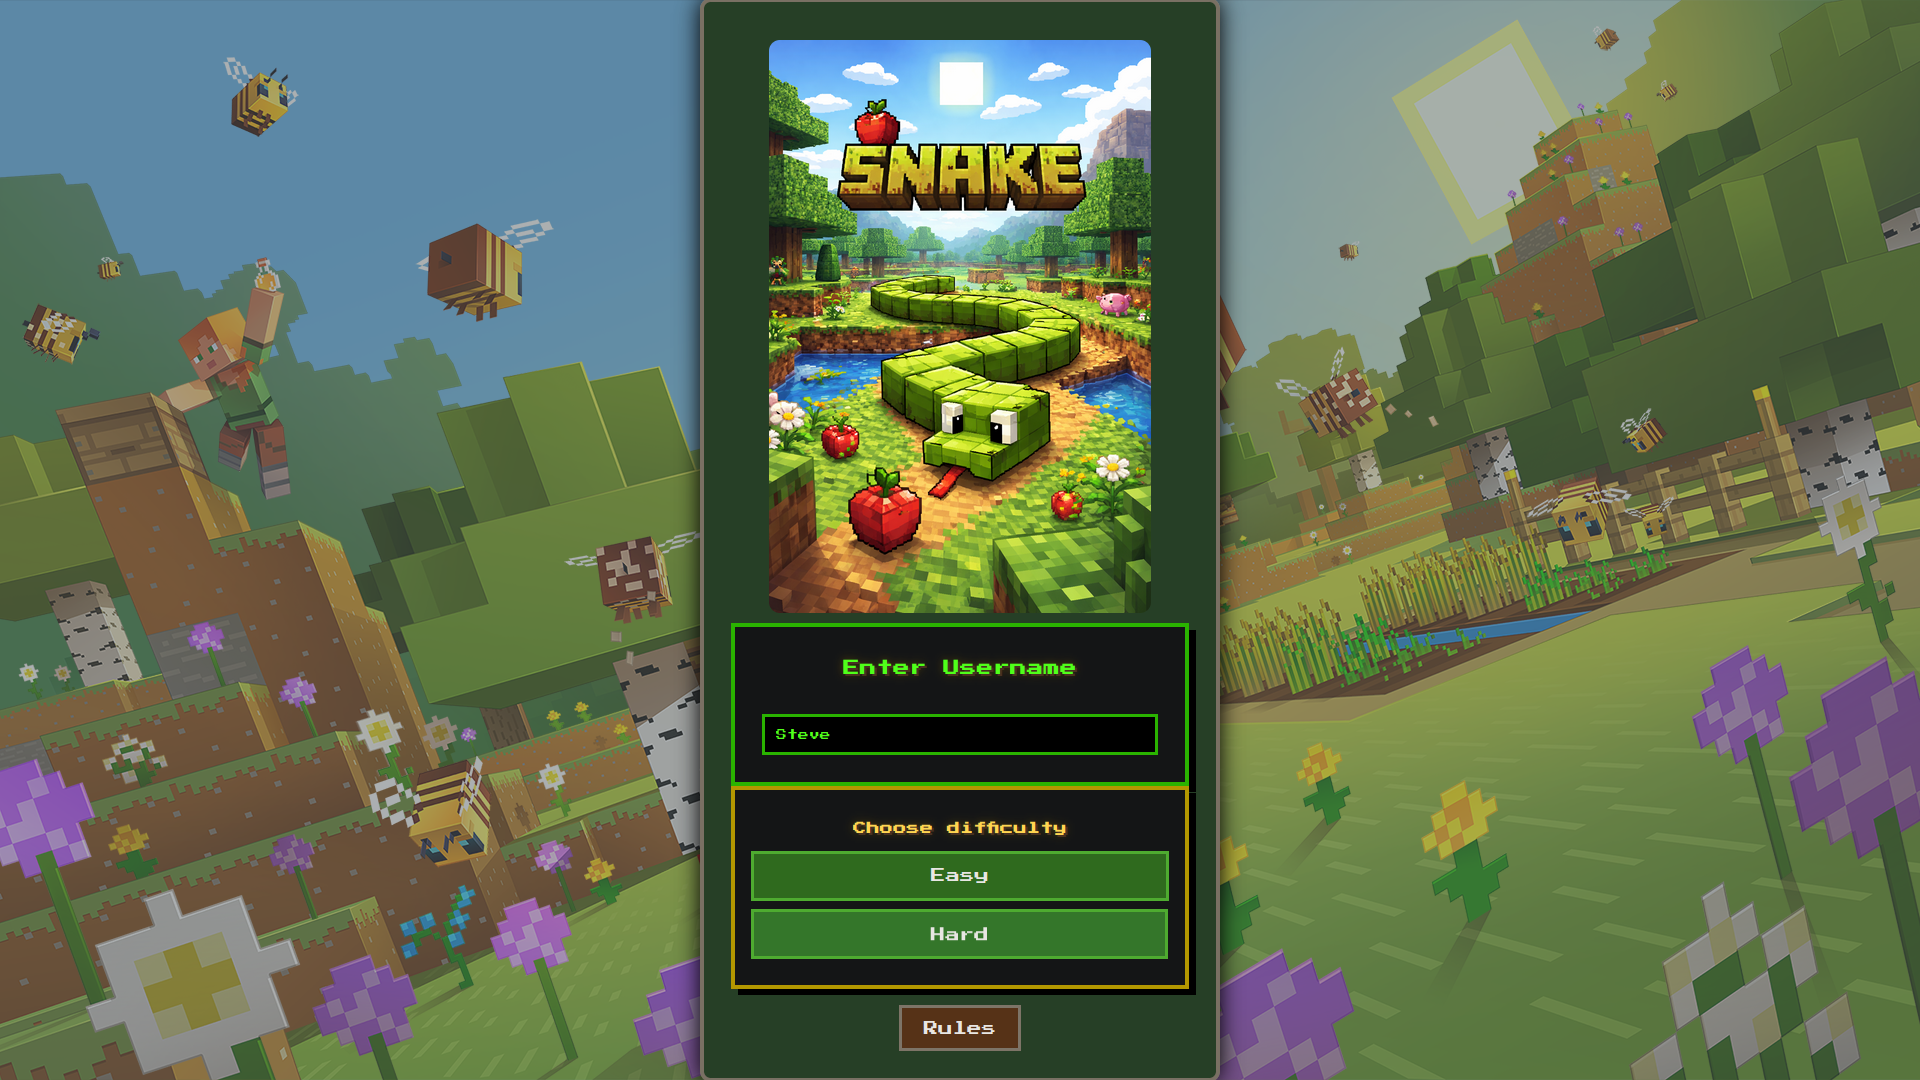
\includegraphics[width=0.95\linewidth]{images/HomeScreen.png}
        \caption{A Screenshot of the Home Screen}
        \label{fig:HomeScreen}
    \end{figure}
    \begin{itemize}
        \item Once a difficulty is selected, the user enters the in-game screen and can start playing.
    \end{itemize}

    \begin{figure}[H]
        \centering
        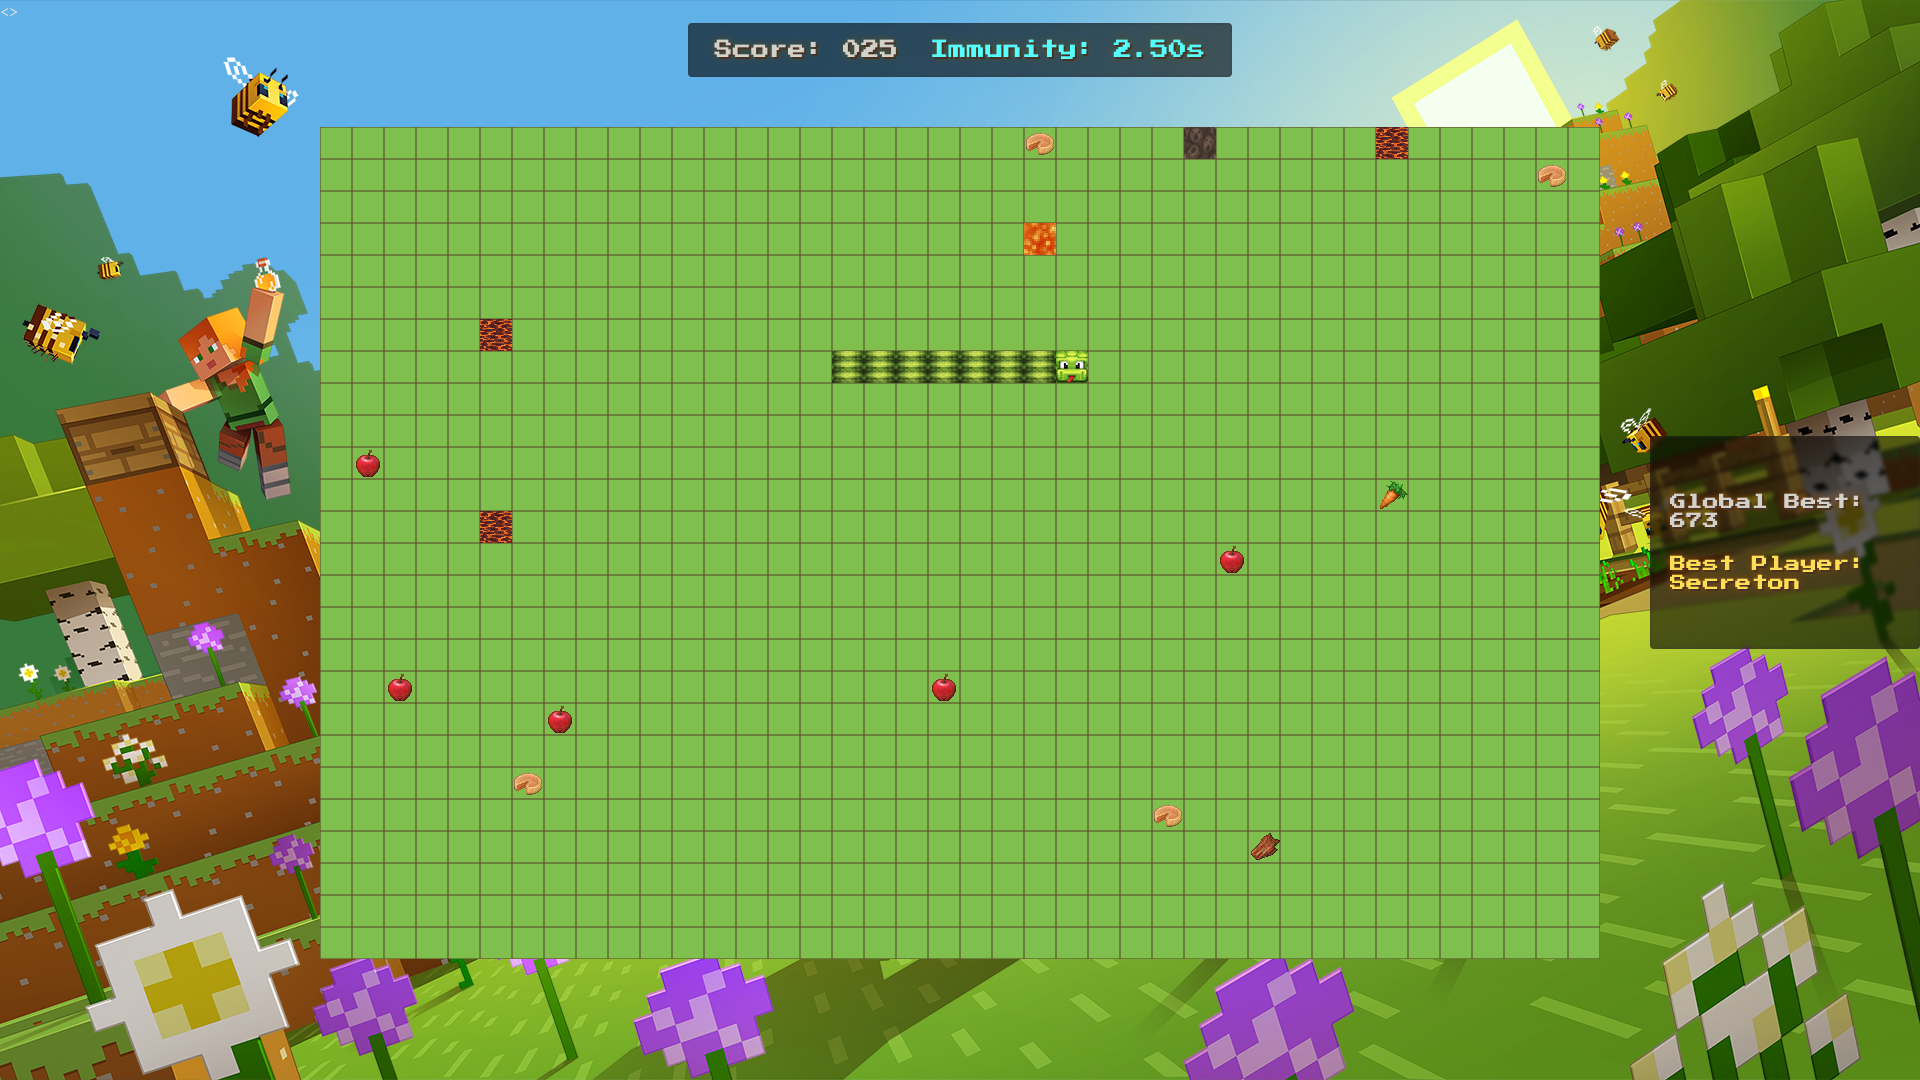
\includegraphics[width=0.95\linewidth]{images/Ingame.png}
        \caption{A Screenshot of the in-game Screen in Hard Difficulty}
        \label{fig:InGame}
    \end{figure}

    \begin{itemize}
        \item Once the player dies for whatever reason, an end screen pops up displaying a humorous death message, cause of the death, Final Score, the time survived, and a humorous status.
        \item The user can choose to return to the home screen or continue playing with the same username and difficulty.
    \end{itemize}

    \begin{figure}[H]
        \centering
        \includegraphics[width=0.95\linewidth]{images/Endscreen.png}
        \caption{A Screenshot of the end screen}
        \label{fig:EndScreen}
    \end{figure}

    \section{External Libraries Used}
    \subsection{Flask}
    Flask \cite{flask_docs}is a lightweight WSGI web application framework. It is designed to make getting started quick and easy, with the ability to scale up to complex applications.

    \begin{itemize}
        \item Flask Version Used: 3.1.3
        \item Python Version Used: 3.10
    \end{itemize}
    In this project Flask is majorly used for three purposes:
    \begin{itemize}
        \item The flask server serves \texttt{index.html} when the user visits the URL (/).
        \item Upon the player’s death, the Flask server retrieves the game state from the frontend as a string, validates it, parses it into JSON and appends it to \texttt{history.txt}.
        \item Whenever the player dies or the webpage loads, the flask server iterates through all the logs present in \texttt{history.txt} to evaluate the highest score among all users and post the highest score and the user with that score to the frontend.
    \end{itemize}

    \subsection{csv}
    Python's \texttt{csv} \cite{csv}module is a built-in library used for reading and writing tabular data in Comma Separated Values (CSV) format. It handles the complexities of CSV parsing, such as properly managing different delimiters, quoting characters, and newline formats.
    
    This project uses the built-in \texttt{csv} module provided by Python 3.10.
    
    In this project the \texttt{csv} Library is used for reading through all the log files when evaluating the highest score among all logs present in \texttt{history.txt}.

    \section{Features Implemented}
    \subsection{Home Screen}
    A modal popup appears when the webpage loads, where 
    \begin{itemize}
        \item The player must choose a difficulty.
        \item The player is prompted to enter a username, which is then validated. The username must not contain any special characters to prevent parsing errors when the Flask server processes the fetched data.
        \item A rules section is also available, which when clicked, pops a modal where the player can read the rules.
    \end{itemize}
    \subsection{Snake movement}
    \begin{itemize}
        \item Movement is controlled using \texttt{WASD} or Arrow keys, implemented through \texttt{keydown} event listeners that capture user input in real time.
        \item All snake cells are maintained in an array, which is rendered on the screen at every frame of the game. During each update cycle, the last cell is removed, and a new head cell is added in the direction of the current movement, effectively simulating the snake’s motion.
    \end{itemize}
    \subsection{Game Frame Rate }
    \begin{itemize}\item A variable \texttt{timestamp} stores the elapsed time since the \texttt{gameLoop} function was last invoked. The \texttt{gameLoop} itself is repeatedly called using JavaScript’s inbuilt \texttt{requestAnimationFrame}, ensuring smooth and frame-synchronised updates.

\item The variable \texttt{basemovementrate} governs the overall update frequency of the game engine, effectively controlling how often the game state is refreshed. In contrast, \texttt{snakemovementrate} specifically determines how frequently the snake advances within the game grid.

\item This separation allows dynamic adjustment of the snake’s speed without affecting the core game loop. For instance, when the snake interacts with obstacles such as SoulSand or BlueIce, \texttt{snakemovementrate} is modified to simulate slowed or accelerated movement, while the base engine continues running at a consistent rate.
    \end{itemize}

    \subsection{Score, Snake Length and Snake Health}

    In this game Score $=$ Snake Health $\neq$ Snake Length.
    \begin{itemize}
        \item Snake Length increases by one whenever a food item is eaten.
        \item Snake health/Score of the player changes based on the food consumed or the effects of obstacles encountered.
        \item Various food items increase the Score/Snakehealth by a varied amount (refer to Table~\ref{tab:FoodType}).
        \item Various obstacles change the Score/SnakeHealth.
    \end{itemize}
    \subsection{Immunity}
    \begin{itemize}
        \item Certain food items provide immunity to the snake for a certain duration (refer to Table~\ref{tab:FoodType}).
        \item When the snake is immune, it remains unaffected from all negative effects i.e. its score and health do not decrease, and it cannot die from colliding with walls or burning in lava.
    \end{itemize}
    \subsection{Game Layout}
    
    \subsubsection{Explanation}
    \begin{itemize}
        \item A centrally placed HTML5 Canvas Element for the game window (refer to Figure~\ref{fig:InGame}).
        \item A Scoreboard displayed at the top of the screen displaying, the current score,
        the duration of immunity left for the player, Overall highscore among all players, The username of the player with the highest score.
    \end{itemize}
    \subsubsection{Implementation}
    \begin{itemize}
        \item A \texttt{<canvas>} element is defined in \texttt{index.html}, and its 2D rendering context is initialized in \texttt{logic.js}. The \texttt{UpdateCanvas} function is responsible for drawing the game state and is called within the \texttt{gameLoop}, which runs once per game frame.
        \item The Scoreboard is updated every 0.25s with the help of \texttt{updateTimers} function, which in turn is called in \texttt{gameLoop}.
    \end{itemize}
    
    \subsection{Food Types and Spawning} 
    \subsubsection{Explanation}
    \begin{itemize}
        \item Various foodtypes have been implemented as listed below:
    \end{itemize}
    \begin{table}[H]
        \centering
        \begin{tabular}{|c|c|c|}
        \hline
        \textcolor{red}{FOOD TYPE}  & \textcolor{red}{HEALTH} & \textcolor{red}{IMMUNITY(in s)}\\
        \hline
        APPLE& 1 & 0  \\
        CARROT& 1 & 0 \\
        PUMPKIN PIE& 4 & 0\\
        GOLDEN CARROT& 5 & 5\\
        GOLDEN APPLE& 5 & 7\\
        ENCHANTED APPLE&10 & 10\\
        \hline
        \end{tabular}
        \caption{Various foodtypes and their functions}
        \label{tab:FoodType}
    \end{table}
    \subsubsection{Implementation}
    \begin{itemize}
        \item A \texttt{Food} class has been implemented and 6 objects have been created of this class with each object having different attributes, The objects are stored in a map and are accessed whenever required.
    \end{itemize}
    \begin{verbatim}
        class Food(){
            constructor(name, health, immunity, img_src){
                //LOGIC HERE
            }
        }
        FOOD_ITEMS = new Map([
            ["APPLE", new Food("APPLE", 1, 0, 0.4, "/static/assets/apple.png")],
            ...
        ])
    \end{verbatim}
    \begin{itemize}
        \item During every frame of the game all the grid cells are iterated over and a randomly generated number is assigned to each cell of the grid using \texttt{Math.random()} in javascript, and if this number exceeds a certain value say $p$, then a food item is spawned in that cell.
        \item $p$ is inversely proportional to the exponent of the number of food items already present on the grid i.e. $p \propto e^{-N}$ where $N$ is the number of food items already present on the grid. Refer to the simplified code below from \texttt{logic.js} .
        
    \end{itemize}
    \begin{verbatim}
    for (let i = 0; i < CANVAS_WIDTH / GRID_WIDTH; i++)
        for (let j = 0; j < CANVAS_HEIGHT / GRID_WIDTH; j++)
            if (
            Math.random() < (object.probability) / (e ** (Food_cells.length))
            )
            Food_cells[Food_cells.length] = { x: i, y: j, type: food_name };
  
    \end{verbatim}
    \vspace{0cm}
    
    \subsection{End Screen}
    \label{sec:EndScreen}
    \begin{itemize}
        \item Whenever the snake dies due to a collision with a wall, its own body, lava, or when its health reaches zero, an endscreen modal pops up displaying a humorous death message, score of the player, cause of the death, Time survived, and an option to either continue playing or go back to home screen.
        \item A \texttt{POST}\cite{fetch_api} request is sent to the flask server at \texttt{/save\_score} with the current game data and the flask server parses the incoming JSON data into a dictionary and appends it to \texttt{history.txt}, Refer to the code from \texttt{logic.js} and \texttt{app.py}
    \end{itemize}
    \begin{verbatim}
        fetch("http://127.0.0.1:5000/save_score", {
            method: "POST",
            body: JSON.stringify({
                // data
            })
        })

        @app.route("/save_score", methods=["POST", "GET"])
        def get_score():
            data = request.get_json()
        with open(history, "a") as file:
        // write
        return message
    \end{verbatim}
    \begin{itemize}
        \item Another \texttt{POST} request is sent to the flask server with game data at \texttt{/highscore.json} to fetch the Global highscore and best player, the flask server parses the incoming JSON and iterates over all the log files in \texttt{history.txt} to get the player with the highest score using a csv reader.
    \end{itemize}
    \subsection{Obstacles}
    \subsubsection{Explanation}
    \begin{itemize}
        \item Various obstacles with different effects have been implemented as listed below:
    \end{itemize}
    \begin{table}[H]
        \centering
        \begin{tabular}{|c|l|}
            \hline
             \textcolor{red}{OBSTACLE}&\textcolor{red}{EFFECT}  \\
             \hline
             ROTTEN FLESH& The Score goes down by 1 for 5 seconds after consumption. \\
             LAVA & Immediate death of the player.\\
             MAGMA & Reduction of score by 0.5 every frame the snake is in contact with the block.\\
             SOUL SAND & Slows down the snake by half of its default speed. \\
             BLUE ICE & Speeds the block by twice its default speed.\\
             \hline
        \end{tabular}
        \caption{Caption}
        \label{tab:Obstacles}
    \end{table}
    \subsubsection{Implementation}
    \begin{itemize}
        \item A super class \texttt{Obstacle} is made with sub classes inherriting this class.
        \item Subclasses \texttt{RottenFlesh}, \texttt{Lava}, \texttt{Magma}, \texttt{SoulSand}, and \texttt{BlueIce} inherit from the superclass constructor along with the methods \texttt{isActive} and \texttt{isPassiveActive}. Each subclass implements its own \texttt{effect} function, which defines the specific behavior or impact associated with that entity.
    \end{itemize}
    \begin{verbatim}
        class Obstacle(){
            constructor(name, row, column, img_src){
                // CODE
            }
        }
        class RottenFlesh extends Obstacle(){
            constructor(){
                super();
            }
            // CODE
        }
    \end{verbatim}
    \begin{itemize}
        \item The spawning of obstacles follows a similar approach to food items, with one key difference: a new instance of the corresponding subclass is created each time an obstacle spawns. In contrast, food items are retrieved from a predefined lookup map of existing objects.
    \end{itemize}
    \subsection{Administration}
    \label{sec:Administration}
    \subsubsection{Explanation}
    \texttt{admin.sh} is used to manage and administer the logs stored in \texttt{history.txt}. The administrator can perform the following operations:
    \begin{itemize}
        \item View user-specific statistics, including recent games or overall metrics such as mean score, average survival time, and the distribution of different death types.
        \item Sort log entries based on timestamp, username, or score.
        \item Delete entries based on username, timestamps, or invalid record formats in \texttt{history.txt}.
        \item Perform log rotation by compressing \texttt{history.txt} and storing archived logs in the \texttt{archive/} directory.
        \item View all the unique usernames present in the log file.
    \end{itemize}
    \subsubsection{Implementation}
    \begin{itemize}
        \item User-specific statistics are computed using \texttt{awk} by parsing each log entry and filtering based on the username.
        \item Sorting of log entries is performed using the built-in \texttt{sort} utility in Bash.
        \item Deletion of log entries is handled using a combination of \texttt{sed} and \texttt{awk}.
        \item Log rotation is performed using \texttt{logrotate}. The file \texttt{administration/logrotate.conf} is dynamically generated by \texttt{admin.sh}, which first checks whether \texttt{history.txt} exceeds 10\,KB. Upon rotation, older logs are compressed and stored in the \texttt{archive/} directory, retaining up to four archived files while preserving the last 10 lines in \texttt{history.txt}. The file \texttt{administration/logrotate.state} maintains state information to prevent redundant or incorrect rotations.
        \item Extraction of all unique usernames is performed using \texttt{awk}.
        \item Viewing all unique usernames is done with the help of \texttt{awk}.
    \end{itemize}
    \section{Directory structure}
    
    \begin{verbatim}
                
            .
            |-- administration
            |   |-- deletebytimestamp.awk
            |   |-- logrotate.conf
            |   |-- logrotate.state
            |   `-- userstats.awk
            |-- admin.sh
            |-- app.py
            |-- archive
            |   |-- history.txt.1.gz
            |   |-- history.txt.2.gz
            |   |-- history.txt.3.gz
            |   `-- history.txt.4.gz
            |-- history.txt
            |-- README.md
            |-- requirements.txt
            `-- static
                |-- assets
                |   `--fonts
                |-- index.html
                |-- logic.js
                `-- styles.css
\end{verbatim}
\subsection{Short description of each file}
\begin{itemize}
    \item \verb|administration/deletebytimestamp.awk|: Implements filtering logic for deleting entries in \verb|history.txt| based on the specified timestamps.
    \item \verb|administration/logrotate.conf|: Configuration file for rotating \texttt{history.txt}; initially empty and populated dynamically by \texttt{admin.sh}.
    \item \verb|administration/logrotate.state|: Maintains logrotate’s state information (e.g., last rotation times) to prevent redundant or incorrect rotations of \texttt{history.txt}.
    \item \verb|administration/userstats.awk|: Calculates various user-specific stats like Mean Score, Mean Time Survived, fraction of specific death types.
    \item \verb|admin.sh|: Handles the entire administration of \texttt{history.txt} by using the files in \texttt{administration} directory.
    \item \verb|app.py|: Handles entirety of backend logic.
    \item \verb|archive/|: Stores upto 4 compressed log files after performing logrotation.
    \item \verb|history.txt|: Stores log files of the game data in specific format.
    \item \verb|requirements.txt|: Stores all the external dependencies in python required to run the game.
    \item \verb|static/assets|: Images and fonts used in the frontend are stored in this directory.
    \item \verb|static/index.html|: Serves as the entry point of the frontend, defining the DOM structure and integrating external styles and scripts.
    \item \verb|static/styles.css|: Provides the styling layer for the frontend, managing layout, theming, and visual consistency across components.
    \item \verb|static/logic.js|: Encapsulates the core client-side behaviour, including event handling, state updates, and real-time interaction logic.
\end{itemize}
\section{Three Layer Communication}
This project contains Three layers:
\begin{itemize}
    \item The frontend (JavaScript + HTML5 Canvas)
    \item The backend (Python/Flask)
    \item Administration (Bash)
\end{itemize}
The three layers communicate as follows:

\vspace{0.2cm}

\texttt{Browser(JS)}$\rightarrow$ \texttt{POST /save\_score or /highscore.json}$\rightarrow$\texttt{Flask}$\rightarrow$\texttt{history.txt}$\leftarrow$\texttt{Bash}.
\vspace{0.3cm}

Refer to section~\ref{sec:EndScreen} to understand how the frontend communicates with the backend.

The bash script doesn't communicate with either of the frontend or the backend, it is unaware of the existence of the frontend or the backend. Refer to section~\ref{sec:Administration} to understand how the administration works.

The format of logs in \texttt{history.txt} is chosen to be of the form shown with and example below:

\begin{verbatim}
    27/04/2026, 20:27:59|Secreton|170|BODY|85.00s
\end{verbatim}

This format was chosen to easily parse with $|$ as the delimiter.

\section{Design and Architectural Decisions}
\begin{itemize}
    \item The system follows a three-layer architecture consisting of a JavaScript-based frontend, a Flask backend, and a Bash-based administration layer. Each layer is designed to be independent, ensuring clear separation of concerns and ease of maintenance.

\item The frontend handles all user interaction, rendering, and game logic using an HTML5 Canvas, allowing real-time updates and smooth gameplay. The backend, implemented using Flask, acts as an intermediary responsible for validating, processing, and persisting game data into \texttt{history.txt}. This ensures that the frontend remains lightweight and does not directly manage storage.

\item The administration layer operates independently of both frontend and backend, interacting only with stored logs. This design choice enables offline analysis and management without affecting the running application.

\item Game logic is further optimized by decoupling the game loop from snake movement, allowing dynamic speed adjustments for specific obstacles. Additionally, a simple text-based logging format with a fixed delimiter was chosen to enable efficient parsing using standard Unix tools such as \texttt{awk}, \texttt{sed}, and \texttt{sort}.

\item Overall, the architecture prioritizes modularity, simplicity, and ease of extensibility while leveraging lightweight technologies across all layers.
\item The \texttt{Food} and \texttt{Obstacle} classes are designed to be extensible, allowing new food items and obstacle types to be added easily without modifying existing logic.
\end{itemize}
\section{Retrospection}
\subsection{Problems faced and how we overcame}
\begin{itemize}
    \item While implementing obstacles that modify the snake’s speed, using a single frame rate for both rendering and movement led to inconsistencies. This was resolved by decoupling the game update rate from the snake’s movement rate.
    \item During the implementation of immunity, collisions with walls required special handling. Since death checks originally occurred after movement, additional pre-collision checks were introduced to prevent unintended deaths and ensure consistent behaviour when the snake is immune.
    \item For short snake lengths (e.g., length 4), self-collision detection caused unintended behaviour. Adjustments to the movement and rendering timing were made to ensure consistent gameplay and eliminate discrepancies between game logic and visual updates.
    \item As the snake grew and occupied more grid space, spawning food and obstacles became increasingly constrained. To address this, spawn rates were adjusted to be inversely proportional (exponentially) to the number of available cells.
    \item Usernames containing special characters caused server-side issues. Input validation was introduced to restrict invalid characters and prevent crashes.
    \item While implementing advancements, a sliding animation was introduced to enhance visual feedback. This required positioning the element initially outside the visible screen area, then smoothly translating it into view to display the advancement, and subsequently moving it back out of the screen once the animation was complete.
\end{itemize}
\subsection{What could have been done if we had 10 more hours}
\begin{itemize}
    \item Add sound effects to the game.
    \item Add more advancements in the game.
    \item Add better animations for the snake.
\end{itemize}
\section{Bibliography and references}

\bibliographystyle{plain}
\bibliography{references}
\end{document}
